\documentclass{article}

\usepackage{amsmath, amsfonts, amssymb}
\usepackage{amsthm}
\usepackage{hyperref}
\usepackage{tikz-cd}
\usepackage{graphicx}
\usepackage{enumitem}

\graphicspath{{graphics/}}

\author{Matthew Dupraz}
\title{Elliptic Curves over $\mathbb{C}$ and over Finite Fields}

\newtheorem{theorem}{Theorem}[section]
\newtheorem{corollary}{Corollary}[theorem]
\newtheorem{lemma}[theorem]{Lemma}
\newtheorem{proposition}[theorem]{Proposition}

\theoremstyle{definition}
\newtheorem{definition}{Definition}[section]
\newtheorem*{notation}{Notation}

\theoremstyle{remark}
\newtheorem*{remark}{Remark}

\newcommand{\proj}{\mathbb{P}}
\newcommand{\F}{\mathbb{F}}
\newcommand{\C}{\mathbb{C}}
\newcommand{\R}{\mathbb{R}}
\newcommand{\Q}{\mathbb{Q}}
\newcommand{\N}{\mathbb{N}}
\newcommand{\Z}{\mathbb{Z}}
\newcommand{\T}{\mathbb{T}}
\newcommand{\chr}{\operatorname{char}}
\renewcommand{\div}{\operatorname{div}}
\newcommand{\im}{\operatorname{im}}
\newcommand{\id}{\operatorname{id}}
\newcommand{\rk}{\operatorname{rk}}
\newcommand{\tr}{\operatorname{tr}}
\newcommand{\res}{\operatorname{res}}
\newcommand{\ord}{\operatorname{ord}}
\newcommand{\End}{\operatorname{End}}
\newcommand{\Hom}{\operatorname{Hom}}
\newcommand{\ts}{\textsuperscript}

\begin{document}

\maketitle
\section{Basic Definitions and Facts}

\subsection{Weierstrass Equation}

Our main interest are \emph{elliptic curves}, which are curves
in $\proj^2$ of genus 1. These are characterized by the
homogeneous equation
\begin{equation}
	\label{weierstrass-eq-1}
	Y^2Z + aXYZ + bYZ^2 = X^3 + cX^2Z + dXZ^2 + eZ^3
\end{equation}
for some $a, b, c, d, e \in \F$.
Setting $U_Z = \{[X, Y, Z] \in \proj^2 \mid Z \neq 0\}$, we can
study the solutions of (\ref{weierstrass-eq-1}) on
$U_Z$ using the change of coordinates $x = X/Z$
and $y = Y/Z$. We obtain the following equation
\begin{equation}
	\label{weierstrass-eq-2}
	y^2 + axy + by = x^3 + cx^2 + dx + e
\end{equation}
We can further simplify this equation with linear
changes of variables. First notice that if $\chr(\F) \neq 2$,
the left hand side can be
written as
\begin{align*}
	y(y + ax + b) &= (y + \frac{1}{2}(ax + b) - \frac{1}{2}(ax + b))
	(y + \frac{1}{2}(ax + b) + \frac{1}{2}(ax + b))\\
	&= (y + \frac{1}{2}(ax + b))^2 - \frac{1}{4}(ax + b)^2
\end{align*}
Hence by replacing $y$ with $y + \frac{1}{2}(ax + b)$ and
collecting the terms in each monomial, we get an equation
of the form
\begin{equation}
	y^2 = x^3 + \alpha x^2 + \beta x + \gamma
\end{equation}
If $\chr(\F) \neq 3$, we can also get rid of the term in 
$x^2$ with a linear change
of variables. replacing $x$ with $x - \frac{1}{3}\alpha$ yields
\begin{align*}
	y^2 &= (x - \frac{1}{3}\alpha)^3 + \alpha(x-\frac{1}{3}\alpha)^2
	+ \beta(x - \frac{1}{3}\alpha) + \gamma\\
	&= x^3 - \alpha x^2 + \frac{1}{3}\alpha^2 x
	- \frac{1}{27}\alpha^3 + \alpha x^2 - \frac{2}{3}\alpha^2 x
	+ \frac{1}{9}\alpha^3 + \beta x - \frac{1}{3}\alpha \beta
	+ \gamma
\end{align*}
Collecting the terms in each monomial, we get an equation of the
form
\begin{equation}
	y^2 = x^3 + Ax + B
\end{equation}
with $A, B \in \F$.
Plugging back the substitutions $x = X/Z$ and $y = Y/Z$, we obtain
the homogeneous equation
\begin{equation}
	Y^2Z = X^3 + AXZ^2 + BZ^3
\end{equation}

\subsection{Singularities}

We suppose $\F$ is algebraically closed.
	
We have that an elliptic curve $V \subset \proj_2(\F)$
is the projective variety
\begin{equation}
	V = V(X^3 + AXZ^2 + BZ^3 - Y^2Z) = V(F)
\end{equation}
We are interested in the case where the curve is smooth.
By the regular preimage theorem, $V$ is smooth if all its points
are non-singular, i.e. if for all $P = [x, y, z] \in V$,
\begin{equation*}
	\nabla F(P) = 
	\begin{bmatrix}
		3x^2 + Az^2\\
		-2yz\\
		2Axz + 3Bz^2 - y^2
	\end{bmatrix}
	\neq 0
\end{equation*}
If $P = [0, 1, 0]$, then 
\begin{equation*}
	\nabla F(P) = 
	\begin{bmatrix}
		0\\
		0\\
		-1
	\end{bmatrix} \neq 0
\end{equation*}
hence the point at infinity is never singular. It follows
that when looking for singularities, we can consider just
the case where $z \neq 0$, since else we have necessarily $x = 0$
and so $P = [0, 1, 0]$. So if there are any singularities of $V$,
they are on $V \cap U_Z$. So $V$ is non-singular precisely when
$V \cap U_Z$ is non-singular. Using the isomorphism
$V \cap U_Z \to W, [X, Y, Z] \mapsto (\frac{X}{Z}, \frac{Y}{Z})$ it
suffices to study singularities on $W = V(x^3 + Ax + B - y^2)
= V(f)$

Let $\Delta = 4A^3 + 27B^2$ be the discriminant of the polynomial
$g(x) = x^3 + Ax + B$, we have the following criteria for the
existence of singularities of $V$.

\begin{proposition}
	\label{prop:singular-determinant}
	W (and equivalently V)
	is non-singular if and only if $\Delta \neq 0$.
\end{proposition}
\begin{proof}
	Suppose there is a point $P = (x_0, y_0) \in W$ that is singular,
	then we have
	\begin{equation*}
		\begin{bmatrix}
			3x_0^2 + A\\
			-2y_0\\
		\end{bmatrix} = 0
	\end{equation*}
	Hence we have that $g'(x_0) = 3x_0^2 + A = 0$ and $y_0 = 0$.
	In particular, since $P \in W$, also 
	$g(x_0) = 0$, and hence since $g(x_0) = g'(x_0) = 0$,
	$x_0$ is a double root of $g$ and so the discriminant
	$\Delta = 4A^3 + 27B^2$ of $g$ is zero.

	Suppose instead that $\Delta = 0$, then $g$ admits a double root
	$x_0 \in \F$ (since we supposed $\F$ algebraically closed)
	which is unique since $g$ is a cubic polynomial.
	Then $P = (x_0, 0) \in V$.
	Furthermore,
	\begin{equation*}
		\nabla f(P) =
		\begin{bmatrix}
			3x^2 + A\\
			0\\
		\end{bmatrix}
	\end{equation*}
	We have that $3x^2 + A = g'(x) = 0$, hence $\nabla f(P) = 0$
	and so $W$ is singular at $P$.
\end{proof}


\section{Elliptic Curves over \texorpdfstring{$\C$}{C}}
\label{sec:over-C}

The goal of this section is to show an elliptic curve is
isomorphic to a torus as a Riemann surface.

First, let's discuss the Riemann surface structure that an elliptic curve has.

\begin{definition}
	The \emph{complex topology} on $\proj^n$ is the quotient topology induced
	by the Euclidean topology on $\C^{n+1}$.
\end{definition}

Throughout this section we will consider $\proj^n$ with the complex topology,
and hence an elliptic curve $E(\C) \subset \proj^2$ will be equipped with
the subspace topology.

\begin{proposition}
	\label{prop:riemann-surf-struct}
	Let $E(\C) \subset \proj^2$ be an elliptic curve, then $E(\C)$ admits
	the structure of a Riemann surface.
\end{proposition}

\begin{proof}
	Let $y^2 - x^3 - ax - b = f(x, y) = 0$ be the equation defining $E(\C)$.
	So for all $P = (x_P, y_P) \in E(\C)$ with $y_P \neq 0$,
	$\frac{\partial f}{\partial y}(P) \neq 0$ and hence by the implicit function
	theorem there exists an open set $V_P \subseteq \C$ containing $x_P$ and an
	analytic function $g_P: V_P \to \C$, such that $g_P(x_P) = y_P$ and
	$f(x, g_P(x)) = 0$ for all $x \in V_P$. 
	Furthermore $U_P = \mathcal{G}(g_P) = (\id\times g_P)(V_P) \subset E(\C)$,
	is an open subset of $E(\C)$.
	Hence we define
	$\phi_P: U_P \to \C, (x, y) \mapsto x$ which is a homeomorphism to its
	image $\phi_P(U_P) = V_P$ (the inverse to which is given by
	$x \mapsto (x, g_P(x))$). Hence $\phi_P$ defines a chart of $E(\C)$.

	For all $P = (x_P, 0) \in E(\C)$ we define the chart $\phi_P: U_P \to \C$
	similarly, except we inverse the roles of $x$ and $y$ in the above reasoning.
	Indeed, $\frac{\partial f}{\partial x}(P) \neq 0$, since $E(\C)$ is smooth,
	hence we get the existence of $V_P \subset \C$ containing $y_P$ and
	$h_P: V_P \mapsto \C$, such that $h_P(y_P) = x_P$ and
	$f(h_P(y), y) = 0$ for all $y \in V_P$. We set
	$U_P := (h_P \times \id)(V_P)$ and 
	$\phi_P: U_P \to \C, (x, y) \mapsto y$.

	Finally, we have yet to define a chart whose domain covers the point at
	infinity $O = [0, 1, 0] \in E(\C)$. To do this, we can look at $E(\C)$ in
	the chart $U_Y$ instead. We get that in this chart, $E(\C)$ is given by
	the equation. 
	\begin{equation*}
		z - x^3 - axz^2 - bz^3 = \tilde f(x, z) = 0.
	\end{equation*}
	We have that $\frac{\partial \tilde f}{\partial z} (O) = 1 \neq 0$, hence we
	can again apply the reasoning from above. We obtain the chart
	$\phi_O: U_O \to \C, [x, 1, z] \mapsto x$ with inverse
	$\phi_0^{-1}: \phi_O(U_O) \to \C, x \mapsto [x, 1, \tilde g(x)]$.

	Now let $P, Q \in E(\C) \setminus \{O\}$, with $y_P \neq 0$ and $y_Q = 0$.
	We have that
	\begin{align*}
		\phi_P \circ \phi_Q^{-1} (y) &= \phi_P(h_Q(y), y) = h_Q(y)\\
		\phi_Q \circ \phi_P^{-1} (x) &= \phi_{Q}(x, g_P(x)) = g_P(x)\\
		\phi_P\circ \phi_O^{-1}(x) &= \phi_P([x, 1, \tilde g(x)])
		= \phi_P\left(\frac{x}{\tilde g(x)},
		\frac{1}{\tilde g(x)}\right) = \frac{x}{\tilde g(x)}\\
		\phi_O\circ \phi_P^{-1}(x) &= \phi_O(x, g_P(x))
		= \phi_O\left(\left[\frac{x}{g_P(x)}, 1, \frac{1}{g_P(x)}\right]\right)
		= \frac{x}{g_P(x)}
	\end{align*}
	All of these transition maps are holomorphic and by transitivity so are
	$\phi_O \circ \phi_Q^{-1}$ and $\phi_Q \circ \phi_O^{-1}$.
	This gives $E(\C)$ the structure of a Riemann surface.
\end{proof}

Let's introduce the definition and some basic properties of elliptic functions.
For the rest of this section,
let $\Lambda \subseteq \C$ be an arbitrary lattice.

\begin{definition}
	An \emph{elliptic function} (relative to the lattice $\Lambda$)
	is a meromorphic function
	$f$ on $\C$, which satisfies
	\begin{equation*}
		f(z + \lambda) = f(z)\qquad\textrm{ for all } \lambda \in \Lambda, z \in \C
	\end{equation*}
\end{definition}

\begin{notation}
	The set of elliptic functions relative to the lattice $\Lambda$ is denoted
	$\C(\lambda)$.
\end{notation}

\begin{remark}
	$\C(\Lambda)$ is a field with the usual operations of 
	addition and multiplication of complex functions.
\end{remark}

\begin{definition}
	A \emph{fundamental parallelogram} for $\Lambda$ is a set of the form
	\begin{equation*}
		D = \{a + r \lambda_1 + s \lambda_2 \mid r, s \in [0, 1)\},
	\end{equation*}
	where $a \in \C$ and $\lambda_1, \lambda_2$ is a basis for $\Lambda$.
\end{definition}

\begin{proposition}
	\label{prop:no-poles}
	An elliptic function with no poles (or no zeros) is constant.
\end{proposition}

\begin{notation}
	For $f \in \C(\Lambda), z \in \C/\Lambda$, we write $f(z), \res_z(f)$ and $\ord_z(f)$ for
	$f(\bar{z}), \res_{\bar{z}}(f)$ and $\ord_{\bar{z}}(f)$ respectively,
	for any one representative
	$\bar{z} \in \C$ of the coset $z$. This is well defined by the
	$\Lambda$-periodicity of $f$.
\end{notation}

\begin{proposition}
	\label{prop:residue}
	Let $f \in \C(\Lambda)$.
	\begin{enumerate}[label=(\alph*)]
		\item $\sum_{z \in \C/\Lambda} \res_z(f) = 0$.
		\item $\sum_{z \in \C/\Lambda} \ord_z(f) = 0$.
	\end{enumerate}
\end{proposition}

Next let us introduce the Weierstrass $\wp$-function, which will serve
as a connecting link between elliptic curves and elliptic functions.

\begin{definition}
	\begin{enumerate}[label=(\alph*)]
		\item
			The Weierstrass
			elliptic function ($\wp$-function),
			is defined by the series
			\begin{equation*}
				\wp(z; \Lambda) = \frac{1}{z^2}
				+ \sum_{\lambda \in \Lambda\setminus\{0\}}
				\left(
					\frac{1}{(z-\lambda)^2} - \frac{1}{\lambda^2}
				\right)
			\end{equation*}
		\item
			The Eisenstein series (of $\Lambda$) of weight $k$,
			where $k \geq 2$ is an integer
			is the series
			\begin{equation*}
				G_k(\Lambda) = \sum_{\lambda \in \Lambda\setminus\{0\}}
				\lambda^{-k}
			\end{equation*}
	\end{enumerate}
\end{definition}

\begin{notation}
	If $\Lambda$ is known from context, we write simply
	$\wp(z)$ and $G_k$ for $\wp(z; \Lambda), G_k(\Lambda)$
	respectively.
\end{notation}

% Theorem VI.3.1
\begin{proposition}
	\label{prop:wp-properties}
	\begin{enumerate}[label=(\alph*)]
		\item	The Eisenstein series $G_k(\Lambda)$ is absolutely convergent
			for all $k \geq 3$.
		\item The series defining the Weierstrass $\wp$-function converges
			absolutely and uniformly on every compact subset of
			$\C\setminus\Lambda$. It defines a meromorphic function on $\C$ with 
			double poles of residue 0 at each lattice point.
		\item The Weierstrass $\wp$-function is an even elliptic function.
	\end{enumerate}
\end{proposition}

\begin{proof}
	\begin{enumerate}[label=(\alph*)]
	\item	Let $\lambda_1, \lambda_2$ be basis vectors of $\Lambda$.
		Let 
		\begin{equation*}
			A_N := \{n\lambda_1 + m\lambda_2 \in \Lambda \mid
			n, m \in \Z, \max(|n|, |m|) = N\}.
		\end{equation*}
		Let also 
		\begin{equation*}
			m = \min\{|a\lambda_1 + b\lambda_2| \mid 
			a, b \in \R, \max(|a|,|b|) = 1\},
		\end{equation*}
		then $m$ is well defined and strictly positive,
		as it's the minimum of a compact subset of $\R$, which does
		not contain zero. We have that
		\begin{equation*}
			\#A_N = (2N + 1)^2 - (2N - 1)^2 = 8N.
		\end{equation*}
		Furthermore, $\min\{|\lambda|, \lambda \in A_N\} \geq Nm$, so we
		get
		\begin{equation*}
			\sum_{\lambda \in \Lambda\setminus 0}\frac{1}{|\lambda|^k}
			\leq \sum_{N=1}^\infty \frac{\#A_N}{\min\{|\lambda|, \lambda \in
			A_N\}^k}
			= \sum_{N=1}^{\infty} \frac{8}{m^kN^{k-1}} < \infty.
		\end{equation*}
	\item
		If $|\lambda| > 2|z|$, then we have that
		\begin{equation*}
			|2\lambda - z| \leq 2|\lambda| + |z| \leq \frac{5}{2}|\lambda|
		\end{equation*}
		and
		\begin{equation*}
			|z - \lambda| = |\lambda|\left|\frac{z}{\lambda} - 1\right| \geq
			\frac{1}{2}|\lambda|.
		\end{equation*}
		These imply that
		\begin{equation*}
			\left| \frac{1}{(z - \lambda)^2} - \frac{1}{\lambda^2}\right|
			= \left| \frac{z(2\lambda - z)}{\lambda^2(z - \lambda)^2}\right|
			\leq 10\frac{|z|}{|\lambda|^3}
		\end{equation*}
		Hence using (a) we see that for $z \in \C \setminus \Lambda$,
		the series for $\wp(z)$ converges absolutely and uniformly on any 
		compact subset of $\C \setminus \Lambda$. It follows that
		the series defines a holomorphic function on $\C \setminus \Lambda$,
		furthermore, it is clear from the series expansion that $\wp$ has
		a double pole with residue $0$ at each point of $\Lambda$.
	\item TO BE ADDED
	\end{enumerate}
\end{proof}

\begin{theorem}
	\label{thm:wp-generates}
	We have that
	\begin{equation*}
		\C(\Lambda) = \C(\wp, \wp')
	\end{equation*}
\end{theorem}

\begin{definition}
	The \emph{Weierstrass $\sigma$-function} (relative to $\Lambda$) is the
	function defined by
	\begin{equation*}
		\sigma(z; \Lambda) = z \prod_{\lambda\in\Lambda\setminus 0}
		\left(1 - \frac{z}{\lambda}\right)
		\exp\left(\frac{z}{\lambda} + \frac{1}{2}\left(\frac{z}{\lambda}\right)^2\right)
	\end{equation*}
\end{definition}

\begin{notation}
	As before, we write just $\sigma(z)$ for $\sigma(z; \Lambda)$ when $\Lambda$
	is clear from context.
\end{notation}

\begin{proposition}
	\label{prop:complex-divisors}
	Let $n_1, \dots, n_r \in \Z$ and $z_1, \dots, z_n \in \C$, such that
	\begin{equation*}
		\sum n_i = 0 \textrm{ and } \sum n_iz_i \in \Lambda.
	\end{equation*}
	Then there exists an elliptic function $f(z) \in \C(\Lambda)$ satisfying
	\begin{equation*}
		\div(f) = \sum n_i(z_i).
	\end{equation*}
\end{proposition}

\begin{proposition}
	\label{prop:diffeq}
	For all $z \in \C \setminus \Lambda$, we have that
	\begin{equation*}
		\wp'(z)^2 = 4\wp(z)^3 - 60G_4\wp(z) - 140G_6
	\end{equation*}
\end{proposition}

\begin{remark}
	We write
	\begin{equation*}
		g_2 = g_2(\Lambda) = 60G_4
		\textrm{ and }
		g_3 = g_3(\Lambda) = 60G_3.
	\end{equation*}
	Then the equation in \ref{prop:diffeq} becomes
	\begin{equation*}
		\wp'(z)^2 = 4\wp(z)^3 - g_2\wp(z) - g_3
	\end{equation*}
\end{remark}

% Proposition VI.3.6
\begin{theorem}
	\label{thm:lattice-curve}
	Let $g_2, g_3$ be the quantities associated to $\Lambda$ as in the above
	remark.
	Let $E/\C$ be the curve given by the equation
	\begin{equation*}
		E: y^2 = 4x^3 - g_2 x - g_3
	\end{equation*}
	then $E$ is an elliptic curve and the map
	\begin{align*}
		\phi: \C/\Lambda &\to E\\
		z &\mapsto 
		\begin{cases}
			[\wp(z), \wp'(z), 1] &\textrm{if } z \not\in \Lambda\\
			[0, 1, 0] &\textrm{if } z \in \Lambda
		\end{cases}
	\end{align*}
	is a complex analytic isomorphism of complex Lie groups.
\end{theorem}

\begin{proof}
	To show $E$ is an elliptic curve, we have to show that it is non-singular.	
	From \ref{prop:singular-determinant} this is the case if and only if
	the determinant $\Delta$ of the polynomial $f(x) = 4x^3 - g_2x - g_3$
	is non-zero, in other words if and only if $f$ has no repeated roots. 
	Let $\{\lambda_1, \lambda_2\}$ be a basis of $\Lambda$,
	let $\lambda_3 = \lambda_1 + \lambda_2$. then since $\wp'$ is
	an odd elliptic function, we have that for $i \in \{1, 2, 3\}$
	\begin{equation*}
		\wp'(\lambda_i/2) = -\wp'(-\lambda_i/2) = -\wp'(\lambda_i/2)
	\end{equation*}
	and hence $\wp'(\lambda_i/2) = 0$. It follows from $\ref{prop:diffeq}$
	that $\wp(\lambda_i/2)$ is a root of $f$. So we need to show that the
	$\wp(\lambda_i/2)$ are all distinct.
	The function $\wp(z) - \wp(\lambda_i/2)$ has a double zero at $\lambda_i/2$,
	since its derivative is $\wp'(z)$ which vanishes at $\lambda_i/2$.
	Using \ref{prop:residue} and \ref{prop:wp-properties}, we deduce that these
	are the only zeroes and hence the $\wp(\lambda_i/2)$ are all distinct.
	Hence $E$ is indeed an elliptic curve.

	The image of $\phi$ is contained in $E(\C)$ by \ref{prop:diffeq}.
	Let $[x, y, 1] \in E(\C)$, then we have that $\wp(z) - x$ is a non-constant
	elliptic function, so by \ref{prop:no-poles}, it has a zero $a \in \C$.
	Hence $\wp(a) = x$ and hence by \ref{prop:diffeq}, 
	\begin{equation*}
		\wp'(a)^2 = f(\wp(a)) = f(x) = y^2.
	\end{equation*}
	It follows that $\wp'(a) = \pm y$, hence by replacing $a$ with $-a$ in
	the case $\wp'(a) =-y$, we get that $\wp'(a) = y$.
	Hence $\phi(a) = [x, y, 1]$. This shows the surjectivity of $\phi$.

	Now to show injectivity, suppose $z_1, z_2 \in \C$ are such that
	$\phi(z_1) = \phi(z_2)$. Suppose $z_1 \not\equiv -z_1 \mod \Lambda$.
	The function $\wp(z) - \wp(z_1)$ admits the roots $z_1, -z_1, z_2$, but being
	of order 2, two of these values are congruent mod $\Lambda$.
	Hence $z_2 \equiv \pm z_1 \mod \Lambda$. But since
	$\wp'(z_1) = \wp'(z_2)$, we get necessarily $z_2 \equiv z_1 \mod \lambda$.
	
	Now, if $z_1 \equiv -z_1 \mod \Lambda$, then
	\begin{equation*}
		\frac{\partial}{\partial z}(\wp(z) - \wp(z_1)) = \wp'(z)
	\end{equation*}
	and $\wp'(z_1) = \wp'(-z_1) = -\wp'(z_1)$ and hence $\wp'(z_1) = 0$.
	It follows that $z_1$ is a double root of $\wp(z) - \wp(z_1)$, which is of
	order 2. Hence $z_2$, being also a root of $\wp(z) - \wp(z_1)$, is
	necessarily congruent to $z_1$ mod $\Lambda$. This shows the injectivity
	of $\phi$.

	Now we will show $\phi$ is an isomorphism of Riemann surfaces.
	Denote by $\xi: \C \mapsto \C/\Lambda$, the quotient map.
	Then the charts of $\C/\Lambda$ are given by local sections of $\xi$.
	Let $z \in \C$ and $U \ni (x, y)$ an open set such that 
	$\xi\vert_U$ is injective. Let $\psi$ be a chart of $E(\C)$
	which we can suppose (up to shrinking $U$) to be defined on
	$\phi(\xi(U))$.
	Depending on the value of $P = \phi(\xi(z))$, $\psi$ will be of one of the
	three forms as described in the proof of 
	Proposition \ref{prop:riemann-surf-struct}.
	We get that
	\begin{equation*}
		\psi\circ\phi\circ\xi = 
		\begin{cases}
			\wp &\textrm{ if } P \neq O\textrm{ and }\wp'(z) \neq 0\\
			\wp' &\textrm{ if } P \neq O\textrm{ and }\wp'(z) = 0\\
			\frac{\wp}{\wp'} &\textrm{ if }P = O
		\end{cases}
	\end{equation*}
	and hence $\psi\circ\phi\circ\xi$ is holomorphic (and seen as a map to its
	image, it is bijective, and hence biholomorphic). It follows that
	$\phi$ is biholomorphic and hence an isomorphism of Riemann surfaces.
	
	Finally, we want to show that $\phi$ is a group homomorphism.
	Let $z_1, z_2 \in \C$, then from \ref{prop:complex-divisors}, there exists
	a function $f \in \C(\Lambda)$ with divisor
	\begin{equation*}
		\div(f) = (z_1 + z_2) - (z_1) - (z_2) + (0)
	\end{equation*}
	Now, by \ref{thm:wp-generates}, we can write $f(z) = F(\wp(z), \wp'(z))$ for
	some rational function $F(X, Y) \in \C(X, Y)$. We can see $F$ in
	$\C(E)$ and hence $f = F \circ \phi$. It follows that
	\begin{equation*}
		\div (F) = (\phi(z_1 + z_2)) - (\phi(z_1)) - (\phi(z_2)) + (0)
	\end{equation*}
	By Proposition \ref{missing-reference}, it follows that
	\begin{equation*}
		\phi(z_1 + z_2) = \phi(z_1) + \phi(z_2)
	\end{equation*}
\end{proof}

The following theorem (which we will not prove) gives the converse to \ref{thm:lattice-curve}

% Theorem VI.5.1
\begin{theorem}
	\label{thm:curve-lattice}
	Let $E/\C$ be a non-singular curve given by the equation
	\begin{equation*}
		E: y^2 = 4x^3 - ax - b.
	\end{equation*} 
	Then there exists a lattice
	$\Lambda \subseteq \C$ unique up to homothety, such that
	$a = g_2(\Lambda)$ and $b = g_3(\Lambda)$
\end{theorem}

Since any elliptic curve is isomorphic to a curve given by an equation as in
\ref{thm:curve-lattice}, we deduce that all curves are homeomorphic
to a torus $\T^2$. This allows us to calculate its homology groups.

The torus can be given a $\Delta$-complex structure
as in Figure \ref{fig:torus-delta}.
\begin{figure}[h]
	\centering 
	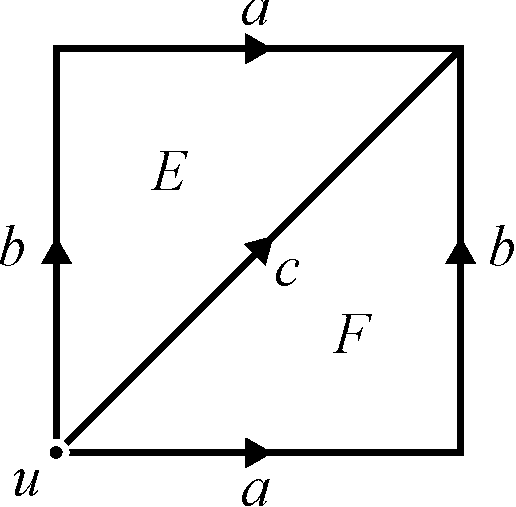
\includegraphics[width=0.4\columnwidth]{torus-delta.pdf}
	\caption[torus-delta]{$\Delta$-complex structure of a torus}
	\label{fig:torus-delta}
\end{figure}
The associated chain complex for taking simplicial homology is 
\begin{equation*}
	\begin{tikzcd}[row sep=tiny]
	\cdots & 0 & {E\Z \oplus F\Z} & {a\Z\oplus b\Z\oplus c\Z} & u\Z & 0 \\
	&&& {a,b,c} & 0 \\
	&& {E,F} & {a +b-c}
	\arrow["\partial_1", from=1-4, to=1-5]
	\arrow["\partial_2", from=1-3, to=1-4]
	\arrow[from=1-5, to=1-6]
	\arrow[from=1-2, to=1-3]
	\arrow[from=1-1, to=1-2]
	\arrow[maps to, from=3-3, to=3-4]
	\arrow[maps to, from=2-4, to=2-5]
\end{tikzcd}
\end{equation*}
Hence we get that
\begin{align*}
	H_0(\T^2) &\cong \Z,\\
	H_1(\T^2) &= \ker \partial_1 / \im \partial_2
	= a\Z \oplus b\Z \oplus c\Z / (a + b - c)\Z \cong \Z^2,\\
	H_2(\T^2) &= \ker \partial_2 = (E-F)\Z \cong \Z,
\end{align*}
and $H_n(\T^2) = 0$ for $n \geq 3$.
We deduce that the associated Betti numbers are
\begin{align*}
	b_0(\T^2) &= \rk(\Z) = 1,\\
	b_1(\T^2) &= \rk(\Z^2) = 2,\\
	b_2(\T^2) &= \rk(\Z) = 1,
\end{align*}
and $b_n(\T^2) = 0$ for $n \geq 3$.

\section{Weil Conjectures}
\label{sec:finite-fields}

For this section we fix a prime $p$ and $q$ a power of $p$.
We suppose throughout this section that $\chr(K) = p$.

In this section we will state the Weil conjectures and prove them in the
case of elliptic curve.

If $K$ is of characteristic $p$,
it contains a unique subfield of order $p^n$ for any $n \in \N$ (see
course \emph{Rings and Fields}), we will denote this subfield by $\F_{p^n}$.
We will be studying the set of
$\F_{q^n}$-rational points of a projective variety.

\begin{definition}
	Let $V/\F_q$ be a projective variety.
	The zeta function of $V/\F_q$ is defined as the power series
	\begin{equation*}
		Z(V/\F_q; T) = \exp\left(\sum_{n=1}^\infty (\#V(\F_{q^n}))
		\frac{T^n}{n}\right)
	\end{equation*}
\end{definition}

\begin{notation}
	When $V/\F_q$ is known from context, we write simply $Z(T)$
	instead of $Z(V/\F_q; T)$
\end{notation}

\begin{theorem}[Weil Conjectures]
	\label{thm:weil}
	Let $V/\F_q$ be a smooth projective variety of dimension $N$.
	\begin{enumerate}[label=(\alph*)]
		\item Rationality: $Z(T) \in \Q(T)$. More precisely, 
			there is a factorization
			\begin{equation*}
				Z(T) = \frac{P_1(T)\cdots P_{2n-1}(T)}
				{P_0(T)P_2(T) \cdots P_{2n}(T)},
			\end{equation*}
			where $P_0(T) = 1 - T, P_{2n}(T) = 1 - q^nT$ and for each
			$1 \leq i \leq 2n - 1$, $P_i(T)$ factors (over $\C$) as
			\begin{equation*}
				P_i(T) = \prod_j (1 - \alpha_{ij}T)
			\end{equation*}
		\item Functional Equation: The zeta function satisfies
			\begin{equation*}
				Z\left(\frac{1}{q^NT}\right) = \pm q^{N\frac{\epsilon}{2}}
				T^{\epsilon} Z(T),
			\end{equation*}
			for some integer $\epsilon$ (called the Euler characteristic of $V$)
		\item Riemann Hypothesis: $|\alpha_{ij}| = q^{i/2}$
			for all $1 \leq i \leq 2n - 1$ and all $j$.
		\item Betti Numbers: If $V/\F_q$ is a good reduction mod $p$ of a
			non-singular projective variety $W/K$, where $K$ is a number
			field embedded in the field of complex numbers, then the degree
			of $P_i$ is the $i$\textsuperscript{th} Betti number of the space
			of complex points of $W$. 
	\end{enumerate}
\end{theorem}

We won't define what a ``good reduction" means in general, but we can
look at the case of elliptic curves given by a Weierstrass equation.

If $K$ be a number field (seen as a subfield of its algebraic closure $\cl{K}$)
and $\O$ its ring of integers. Suppose $E$ is an elliptic curve given by a
Weierstrass equation defined over $K$, i.e. $E$ is of the form
\begin{equation*}
	E: y^2 = x^3 + ax + b
\end{equation*}
with $a, b \in K$. We have that $K = \Frac(\O)$ and so we can write
$a = a_1/a_2$ and $b = b_1/b_2$ for some $a_1, b_1 \in \O$, and
$a_2, b_2 \in \O\setminus\{0\}$.
We can decompose the ideal $(a_2b_2)$ into a product of prime ideals.
\begin{equation*}
	(a_2b_2) = \mf{p}_1\dots\mf{p}_s
\end{equation*}
Then choosing a prime ideal
$\mf{p}$ of $\O$ different from $\mf{p}_i$ for any $i$,
we get that $a_2, b_2 \notin \mf{p}$.
Hence we can see $E$ as being defined over $\O_\mf{p}$.
The maximal ideal $\mf{P}$ of $\O_\mf{p}$ is just the image of $\mf{p}$
under the localization. We deduce
\begin{equation*}
	\O_\mf{p}/\mf{P} \cong (\O/\mf{p})_\mf{p} = \O/\mf{p} \cong \F_q,
\end{equation*}
where $q$ is a power of $p$, where $(p) = \mf{p}\cap\Z$.

This gives us a new curve $C$ obtained by reducing $E$ modulo $\mf{P}$.

\begin{equation*}
	C: y^2 = x^3 + \bar{a}x + \bar{b},
\end{equation*}
defined over the residue field isomorphic to $\F_q$.
We say that $C$ is a \emph{good} reduction of $E$ modulo $p$
if it is also smooth. That is the case if and only if its discriminant
\begin{equation*}
	\Delta(C) = 4\bar{a}^3 + 27\bar{b}^2
\end{equation*}
is non-zero. But notice that the discriminant of $C$ is just the residue
of $\Delta(E) = 4a^3 + 27b^2$ modulo $\mf{P}$.
Hence the reduction of $E$ mod $p$ is ``good" if $\Delta(E) \not\in \mf{P}$.
We will show that (d) of \ref{thm:weil} holds for elliptic curves given
by Weierstrass equations in Section
\ref{sec:over-C}.

In the rest of this section, we will prove the Weil conjectures (save part (d))
for the case
of elliptic curves. For that, we will make use of the relation found in
\ref{prop:deg-tr-det}.
In the following proposition we get a formula for $\#E(\F_{q^n})$, which
we will be able to use for proving the Weil conjectures.

\begin{proposition}
	\label{prop:frob-char-poly}
	Let $E/\F_q$ be an elliptic curve, and
	\begin{equation*}
		\phi: E \to E, (x, y) \mapsto (x^q, y^q)
	\end{equation*}
	the $q$\ts{th}-power Frobenius endomorphism.
	Let $\alpha, \beta \in \C$ be the roots of the characteristic polynomial
	of $\phi_l$, that is
	\begin{equation*}
		\det(T - \phi_l) = T^2 - \tr(\phi_l)T + \det(\phi_l),
	\end{equation*}
	then $\alpha, \beta$ are complex conjugates satisfying
	$|\alpha| = |\beta| = \sqrt{q}$. Furthermore, for every $n \geq 1$, we
	have
	\begin{equation*}
		\#E(\F_{q^n}) = q^n + 1 - \alpha^n - \beta^n
	\end{equation*}
\end{proposition}

\begin{proof}
	We have by \ref{prop:frobenius-separable}
	and \ref{thm:preimage-card}
	that
	\begin{equation*}
		\#E(\F_q) = \deg(1 - \phi)
	\end{equation*}
	and from \ref{prop:deg-tr-det}, we have that
	\begin{equation*}
		\det(\phi_l) = \deg(\phi) = q;\\
	\end{equation*}
	For all $m/n \in \Q$, with $p \nmid m$,
	we have using \ref{prop:frobenius-separable} that
	\begin{equation*}
		\det\left(\frac{m}{n} - \phi_l\right)
		= \frac{\det(m - n\phi_l)}{n^2}
		= \frac{\deg(m - n\phi_l)}{n^2} \geq 0
	\end{equation*}
	Hence the polynomial $\det(T - \phi_l)$ is non-negative for $T \in \R$
	(by continuity). If $\alpha$, $\beta$ are the roots of $\det(T - \phi_l)$,
	it follows that $\alpha$, $\beta$ are complex conjugates (they can be
	equal). So $|\alpha| = |\beta|$ and since $\alpha\beta = \det(\phi_l) = q$,
	it follows that $|\alpha| = |\beta| = \sqrt{q}$.

	Now, for $n \geq 1$ the $(q^n)$\ts{th}-power Frobenius endomorphism
	$\phi^n$ satisfies
	\begin{equation*}
		\#E(\F_{q^n}) = \deg(1 - \phi^n) = \det(1 - \phi_l^n)
	\end{equation*}
	We have that
	\begin{equation*}
		\det(T - \phi_l^n) = (T - \alpha^n)(T - \beta^n)
	\end{equation*}
	since the eigenvalues of $\phi_l^n$ are the $n$\ts{th} powers
	of the eigenvalues of $\phi_l$. From 
	\ref{prop:deg-tr-det}, we have that
	\begin{equation*}
		\tr(\phi_l^n) = 1 + \deg(\phi^n) - \deg(1 - \phi^n)
		= 1 + q^n - \#E(\F_{q^n}).
	\end{equation*}
	and hence 
	\begin{equation*}
		\#E(\F_{q^n}) = 1 + q^n - \tr(\phi_l^m)
		= 1 + q^n - \alpha^n - \beta^n.
	\end{equation*}
\end{proof}

At last, we can state and prove the Weil conjectures for the case
of elliptic curves.

\begin{theorem}
	\label{thm:weil-elliptic}
	Let $E/\F_q$ be an elliptic curve. Then there exists an $a \in \Z$ such that
	\begin{equation*}
		Z(T) = \frac{1 - aT + qT^2}{(1-T)(1-qT)}.
	\end{equation*}
	Furthermore,
	\begin{equation*}
		Z\left(\frac{1}{qT}\right) = Z(T)
	\end{equation*}
	and
	\begin{equation*}
		1 - aT + qT^2 = (1 - \alpha T)(1 - \beta T)
	\end{equation*}
	with $|\alpha| = |\beta| = \sqrt{q}$
\end{theorem}

\begin{proof}
	Using the definition of $Z(E/\F_q; T)$, we get
	\begin{align*}
		\log Z(E/\F_q; T) &= \sum_{n=1}^\infty (\#E(\F_{q^n}))\frac{T^n}{n}\\
		&= \sum_{n=1}^\infty (q^n + 1 - \alpha^n - \beta^n)\frac{T^n}{n}
		\qquad \textrm{(\ref{prop:frob-char-poly})}\\
		&= -\log(1 - qT) - \log(1 - T) + \log(1 - \alpha T) + \log(1 - \beta T)
	\end{align*}
	and hence we get
	\begin{equation*}
		Z(E/\F_q; T) = \frac{(1 - \alpha T)(1 - \beta T)}{(1 - T)(1 - qT)},
	\end{equation*}
	which has the desired form.
	Indeed from (\ref{prop:frob-char-poly}), 
	$|\alpha| = |\beta| = \sqrt{q}$, and
	\begin{align*}
		a = \alpha + \beta = \tr(\phi_l) &= 1 + \deg(\phi) - \deg(1 - \phi)\\
		&= 1 + q - \#E(\F_q) \in \Z.
	\end{align*}
\end{proof}

Hence the Weil conjectures are verified for elliptic curves. Notice that
using the notation from theorem \ref{thm:weil},
$\deg P_0 = 1$, $\deg P_1 = 2$, $\deg P_2 = 1$, hence if $C/\F_q$ is a good
reduction of $E/K$, where $K$ is a number field embedded in
the field of complex numbers, we would expect
the Betti numbers of the space of complex points of $E$ 
to coincide with these values, and indeed, as we
will see in the following section, this is indeed the case.


\end{document}
